%%%%%%%%%%%%%%%%%%%%%%%%%%%%%%%%%%%%%%%%%
% Beamer Presentation
% LaTeX Template
% Version 1.0 (10/11/12)
%
% This template has been downloaded from:
% http://www.LaTeXTemplates.com
%
% License:
% CC BY-NC-SA 3.0 (http://creativecommons.org/licenses/by-nc-sa/3.0/)
%
%%%%%%%%%%%%%%%%%%%%%%%%%%%%%%%%%%%%%%%%%

%----------------------------------------------------------------------------------------
%	PACKAGES AND THEMES
%----------------------------------------------------------------------------------------

\documentclass{beamer}

\mode<presentation> {

% The Beamer class comes with a number of default slide themes
% which change the colors and layouts of slides. Below this is a list
% of all the themes, uncomment each in turn to see what they look like.

%\usetheme{default}
%\usetheme{AnnArbor}
%\usetheme{Antibes}
%\usetheme{Bergen}
%\usetheme{Berkeley}
%\usetheme{Berlin}
%\usetheme{Boadilla}
%\usetheme{CambridgeUS}
%\usetheme{Copenhagen}
%\usetheme{Darmstadt}
%\usetheme{Dresden}
%\usetheme{Frankfurt}
%\usetheme{Goettingen}
%\usetheme{Hannover}
%\usetheme{Ilmenau}
%\usetheme{JuanLesPins}
%\usetheme{Luebeck}
\usetheme{Madrid}
%\usetheme{Malmoe}
%\usetheme{Marburg}
%\usetheme{Montpellier}
%\usetheme{PaloAlto}
%\usetheme{Pittsburgh}
%\usetheme{Rochester}
%\usetheme{Singapore}
%\usetheme{Szeged}
%\usetheme{Warsaw}

% As well as themes, the Beamer class has a number of color themes
% for any slide theme. Uncomment each of these in turn to see how it
% changes the colors of your current slide theme.

%\usecolortheme{albatross}
%\usecolortheme{beaver}
%\usecolortheme{beetle}
%\usecolortheme{crane}
%\usecolortheme{dolphin}
%\usecolortheme{dove}
%\usecolortheme{fly}
%\usecolortheme{lily}
%\usecolortheme{orchid}
%\usecolortheme{rose}
%\usecolortheme{seagull}
%\usecolortheme{seahorse}
%\usecolortheme{whale}
%\usecolortheme{wolverine}

%\setbeamertemplate{footline} % To remove the footer line in all slides uncomment this line
%\setbeamertemplate{footline}[page number] % To replace the footer line in all slides with a simple slide count uncomment this line

%\setbeamertemplate{navigation symbols}{} % To remove the navigation symbols from the bottom of all slides uncomment this line
}

\usepackage{graphicx} % Allows including images
\usepackage{booktabs} % Allows the use of \toprule, \midrule and \bottomrule in tables
\usepackage{epstopdf}
\usepackage{tikz}
\usepackage{booktabs} % Allows the use of \toprule, \midrule and \bottomrule in tables
\usepackage[font=small,skip=0pt]{caption}

%----------------------------------------------------------------------------------------
%	TITLE PAGE
%----------------------------------------------------------------------------------------
%\logo{
\includegraphics[width=0.05\textwidth]{../images/utlogo}}
\title[MARATHON A=3]{Electron Scattering on A=3 Nuclei from MARATHON } % The short title appears at the bottom of every slide, the full title is only on the title page

\author{Jason Bane} % Your name
\institute[UTK] % Your institution as it will appear on the bottom of every slide, may be shorthand to save space
{
	University of Tennessee \\ % Your institution for the title page
	\medskip
	\textit{jbane1@vols.utk.edu} % Your email address
}
\date{March 23, 2019} % Date, can be changed to a custom date
\captionsetup{font=small,skip=0pt}




\begin{document}
\begin{frame}
	\titlepage % Print the title page as the first slide
\end{frame}

\addtobeamertemplate{frametitle}{}{%
\begin{tikzpicture}[remember picture,overlay]
\node[anchor=north east,yshift=2pt] at (current page.north east) {
\includegraphics[height=0.8cm]{../images/utlogo}};
\end{tikzpicture}}

%------------------------------------------------------------------
%------------------------------------------------------------------
\begin{frame}
\frametitle{The MARATHON Experiment}
	MeAsurement of $F^n_2/F^p_2, d/u$ RAtios and $A=3$ EMC Effect in Deep Inelastic Electron Scattering off the Tritium and Helium MirrOr Nuclei.
	\vspace{-10pt}
	\begin{columns}[t]
		\column{.45\textwidth} % L column and width
		\begin{figure}
			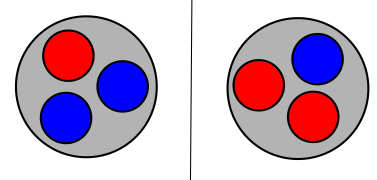
\includegraphics[width =5cm]{../images/mirror}
		\end{figure}
		\vspace{-25pt}
		\begin{figure}
			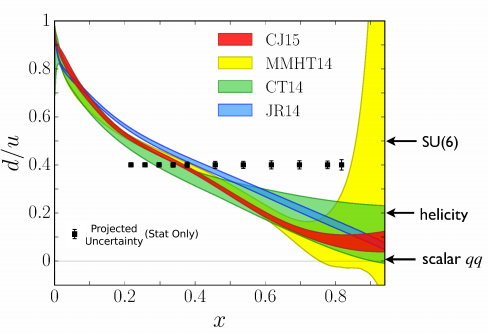
\includegraphics[width=5cm]{../images/d_u}
			\caption{d/u quark distribution ratios}
		\end{figure}
		\column{.55\textwidth} % Right column and width
		\begin{itemize}
			\item Lightest and simplest mirror system
		\begin{itemize}
			\item  Number of protons in $^3H =$ neutrons in $^3He$
		\end{itemize}
			\item Differences in the nuclear effects are small
			\item Improve the current measurement and understanding of $F^n_2/F^p_2$ ratio
			\item Restrict the assumptions and parameters made in the model calculations of the down to up quark distribution ratio
			\item 6 students from 4 universities
		\end{itemize}
	\end{columns}
\end{frame}
%------------------------------------------------------------------
\section{Hall A at JLab}
\begin{frame}
	\begin{block}{Jefferson Lab Hall A}
		\begin{figure}
			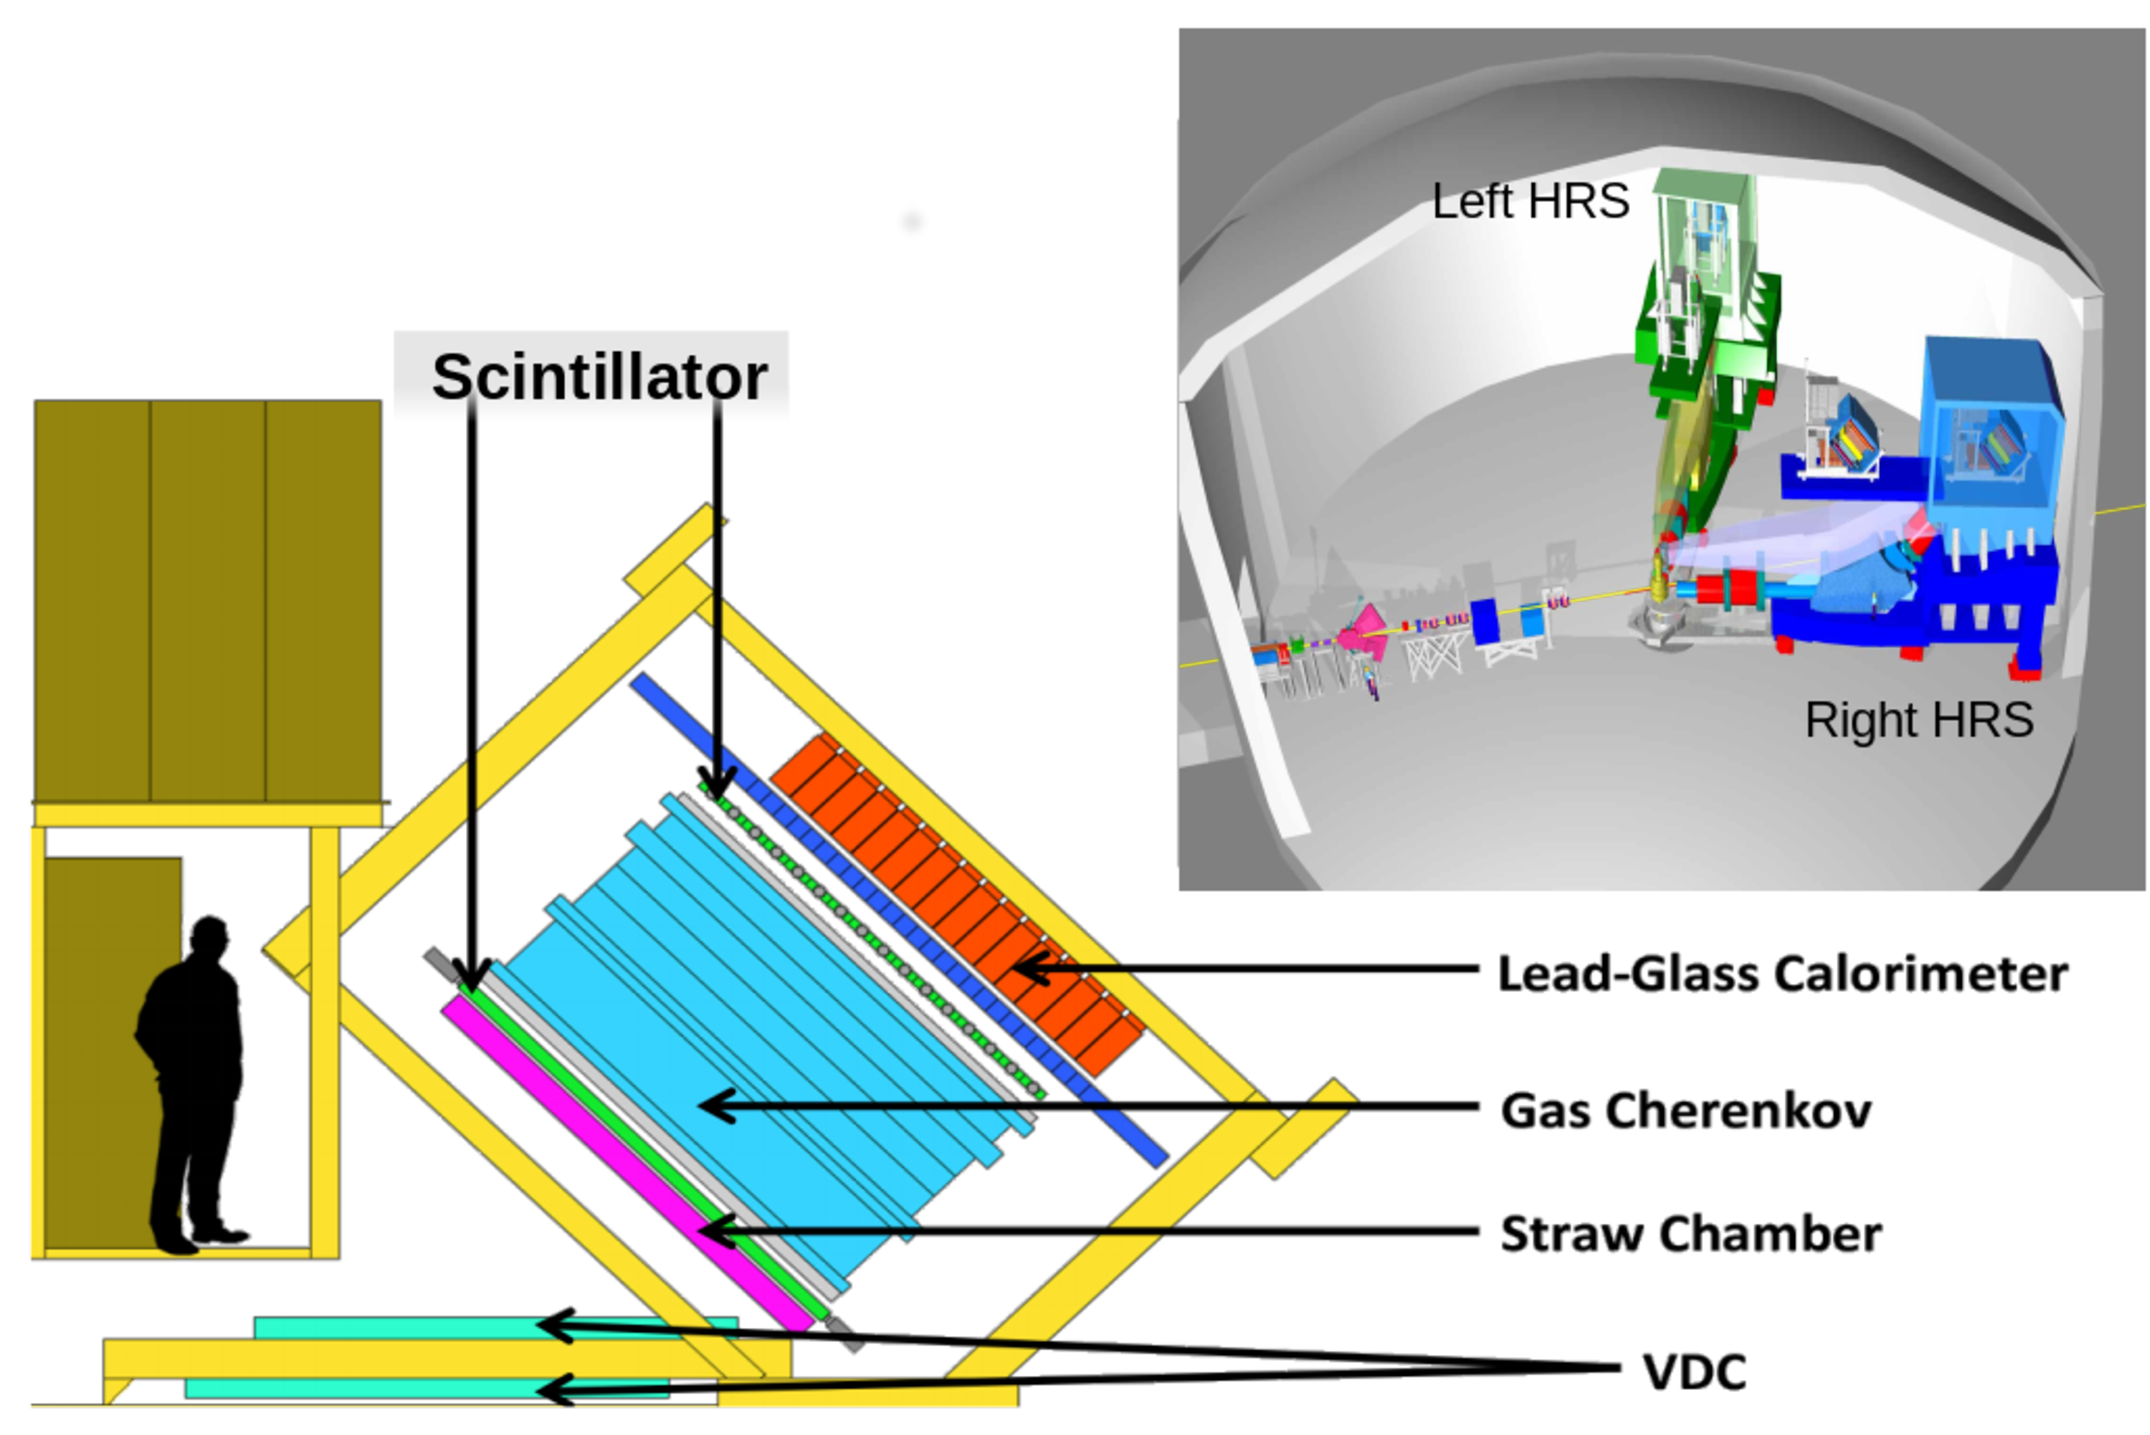
\includegraphics[width=12.0cm]{../images/HallaHRS.pdf}
		\end{figure}
	\end{block}
\end{frame}
%------------------------------------------------------------------

\begin{frame}{Cross Section Analysis}
	\begin{block}{Exacting Yield from Data}
		\centering
		$\frac{d\sigma}{d\Omega dE^\prime} =  \frac{Yield}{Luminosity} = \frac{Ne - BG }{Luminosity *  \epsilon} $
		\begin{itemize}
			\item Luminosity $\equiv$ \# of electrons per scattering centers, needs correction due to density changes
			\item $\epsilon = $ efficiencies
			\item  BG $ = $ background
		\end{itemize}
	\end{block}	
	\begin{block}{Cross section by Monte carlo ratio}	
		$ Yield_{data} = \frac{\left(N_e - BackGround\right)}{Efficency } =  \textit{L} *\sigma^{data} * \left( \Delta E^\prime \Delta \Omega\right)*  A \left(E^\prime \theta \right)$
		$ Yield_{MC} = \textit{L} *\sigma^{mod} * \left( \Delta E^\prime \Delta \Omega\right)*  A \left(E^\prime \theta \right)$
		\centering $ \frac{d\sigma}{d\Omega dE^\prime} = \sigma^{mod} * \left[\frac{Yield_{data} \left( 
			E^\prime,\theta\right)} {Yield_{MC}\left(E^\prime,\theta\right)}\right] $
	\end{block}	
\end{frame}
%------------------------------------------------------------------
\begin{frame}{The efficiency in electron selection}
	\begin{block}{Counting Electrons}
		\begin{columns}
			\column{0.35\textwidth}
			\begin{itemize}
 		 		\setlength{\parskip}{0pt}
				\setlength{\itemsep}{0pt plus 1pt}
				\item Electron ID is done via the Cherenkov and two layers of a total calorimeter.
				\item Deposit large percentage of its energy into the total calorimeter system.
				\item Trigger significant amount of cherenkov radiation
			\end{itemize}		
			\column{0.55\textwidth}
			\begin{figure}
					\textbf{Cherenkov vs. Total energy absorbed}
					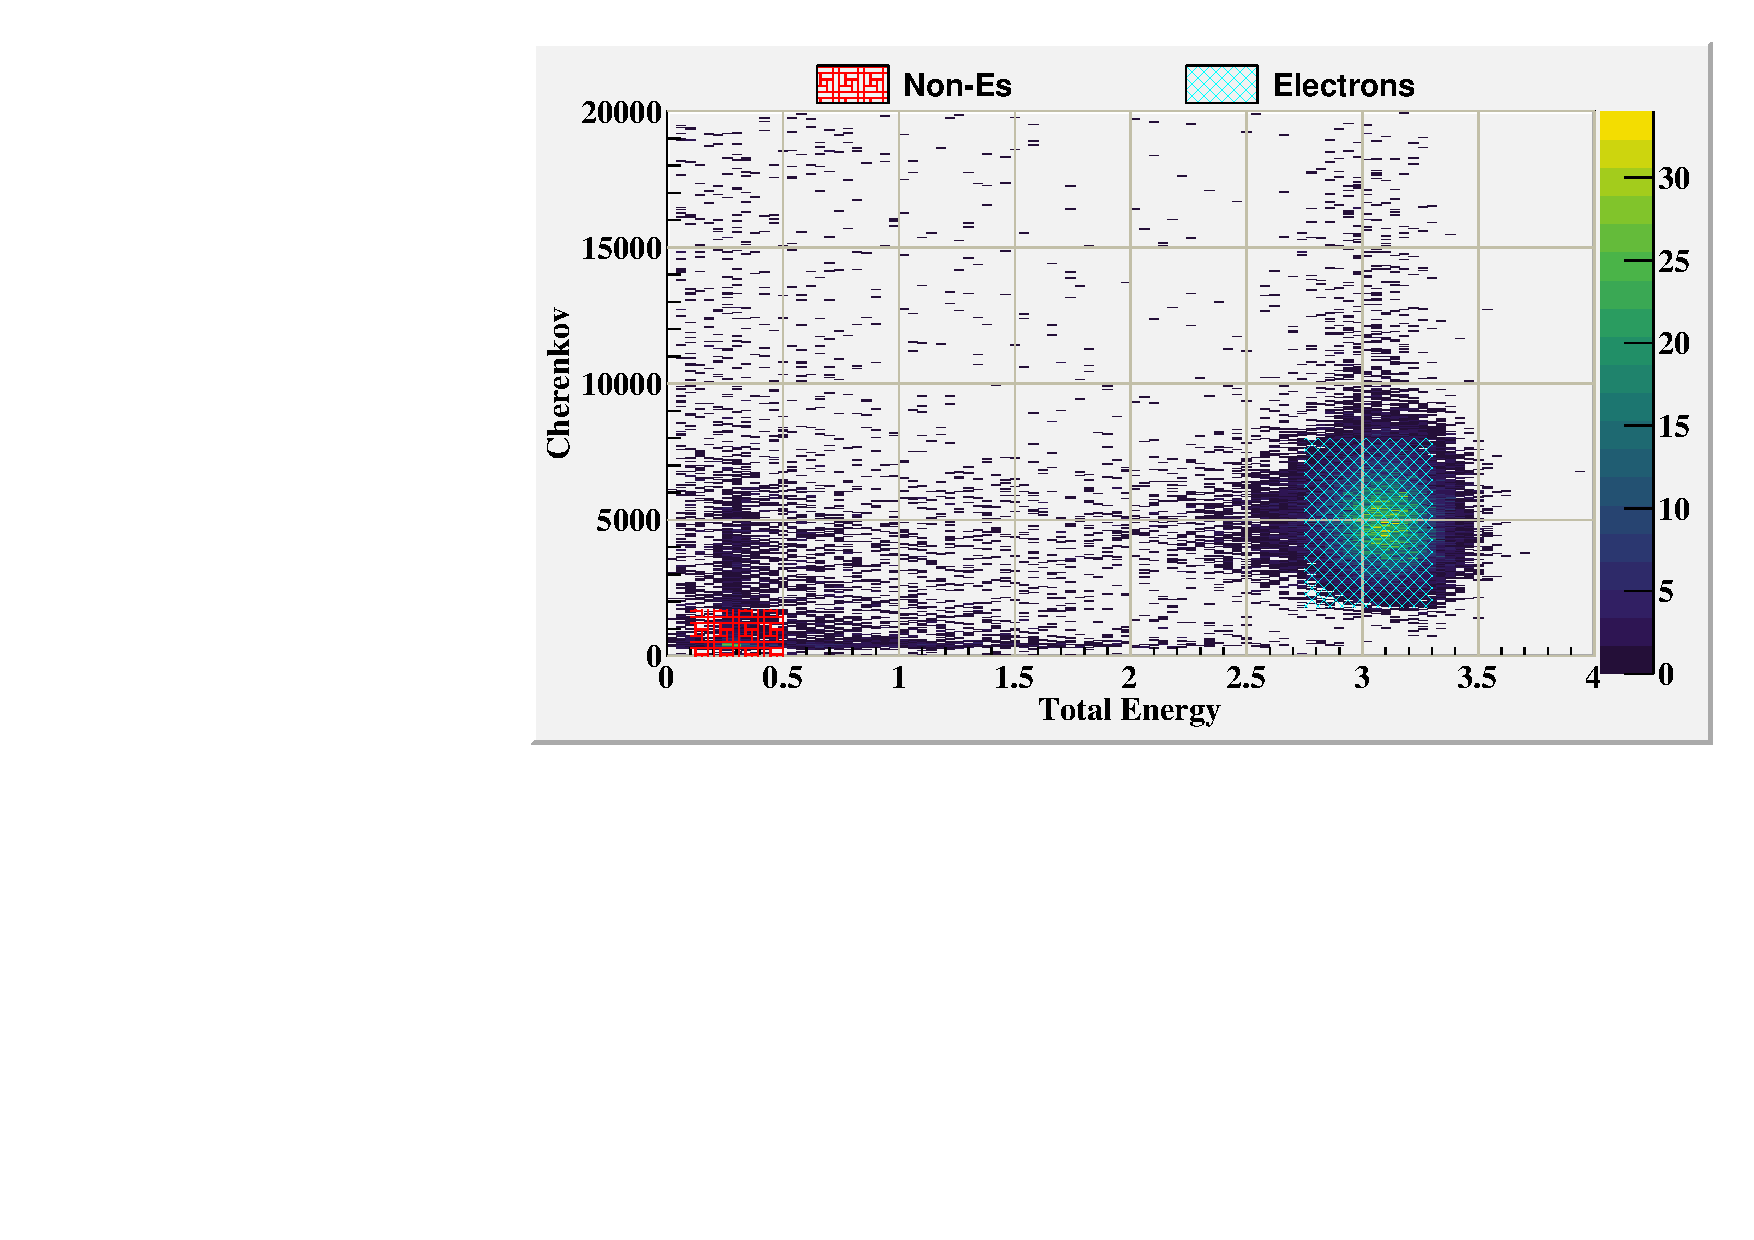
\includegraphics[width=7.0cm]{../images/PID_2d.pdf}
			\end{figure}
		\end{columns}
	\end{block}
\end{frame}
%------------------------------------------------------------------

\begin{frame}{Efficiency of the selection}
	\begin{block}{}
		\begin{columns}
			\column{0.45\textwidth}
			\vspace{-18pt}
			\begin{figure}
				\textbf{First and second layer of calorimeter with electron and non-electron sampling}
				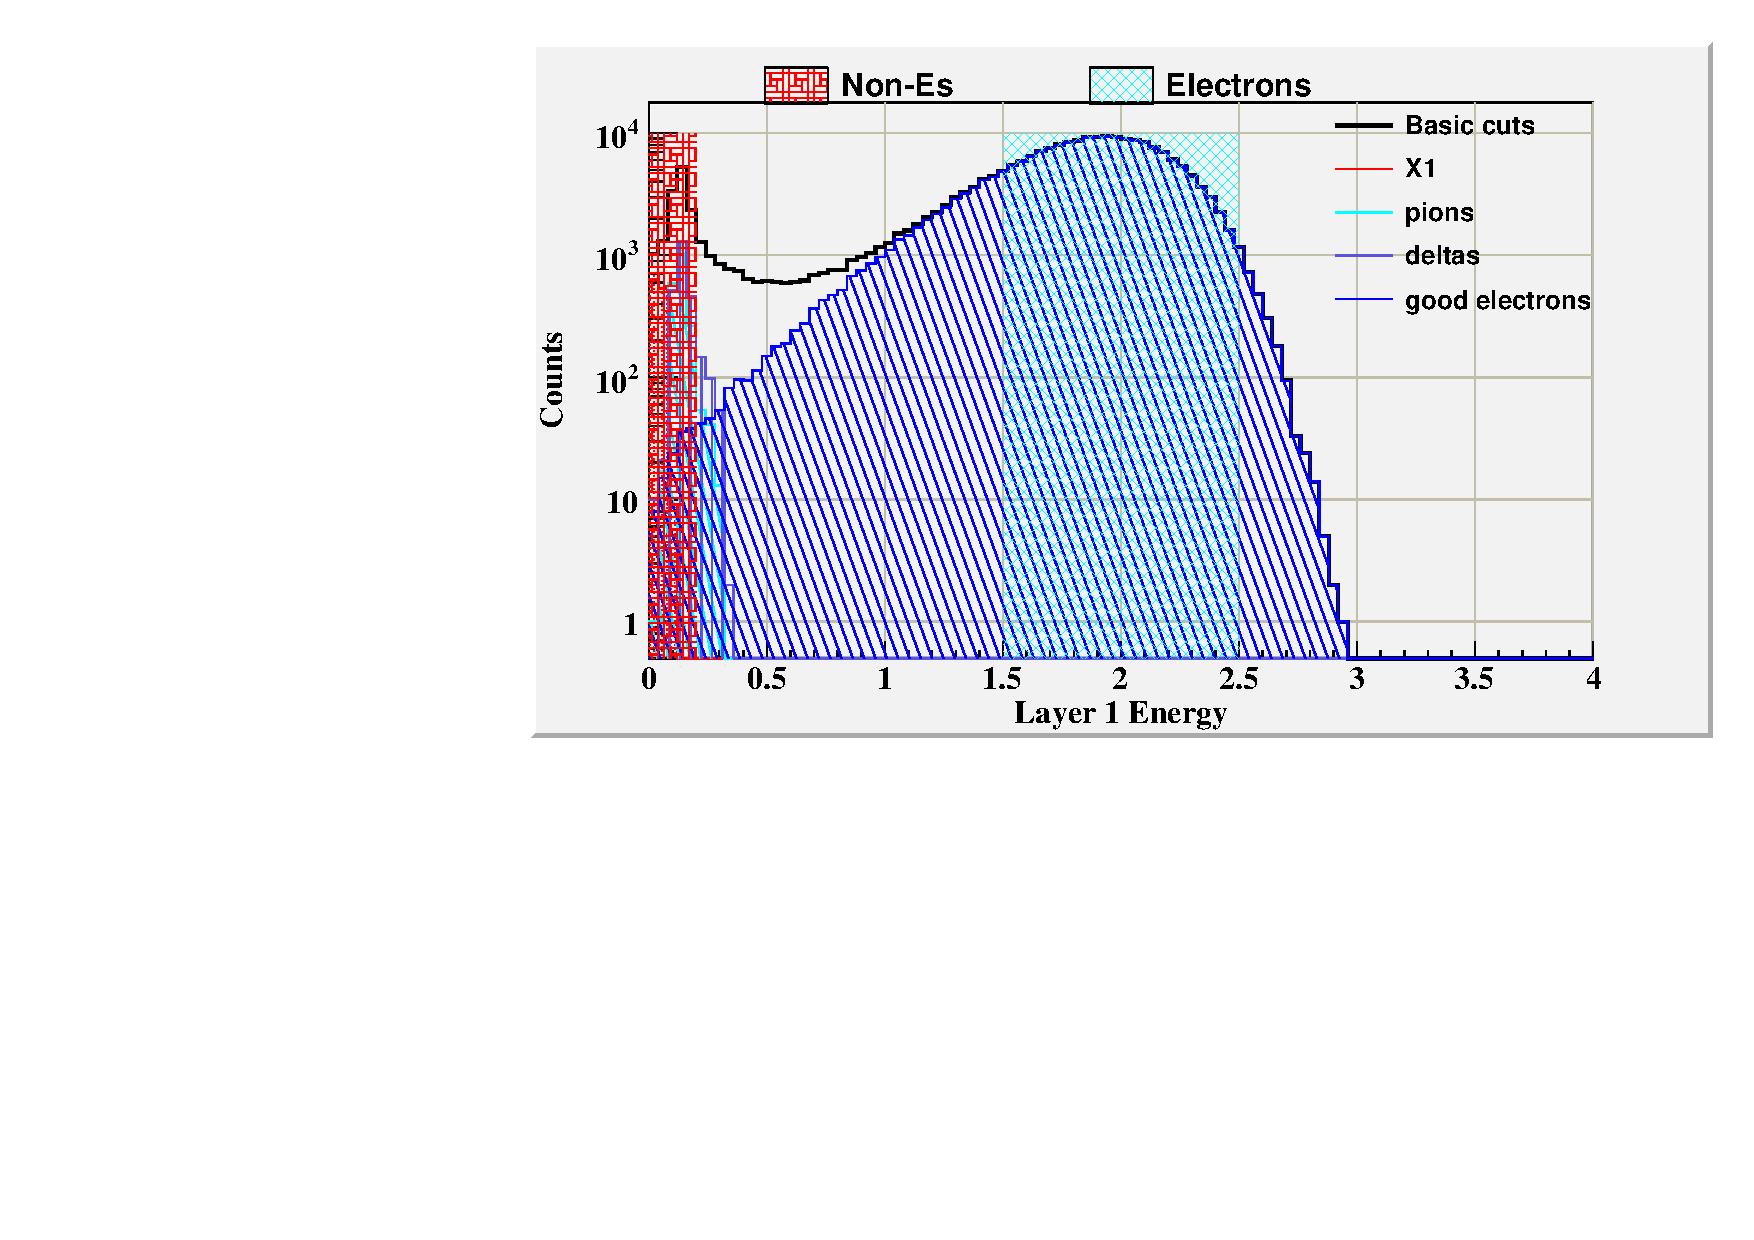
\includegraphics[width=4.50cm]{../images/Lprl1.pdf}
			\end{figure}
			\vspace{-23pt}
			\begin{figure}
				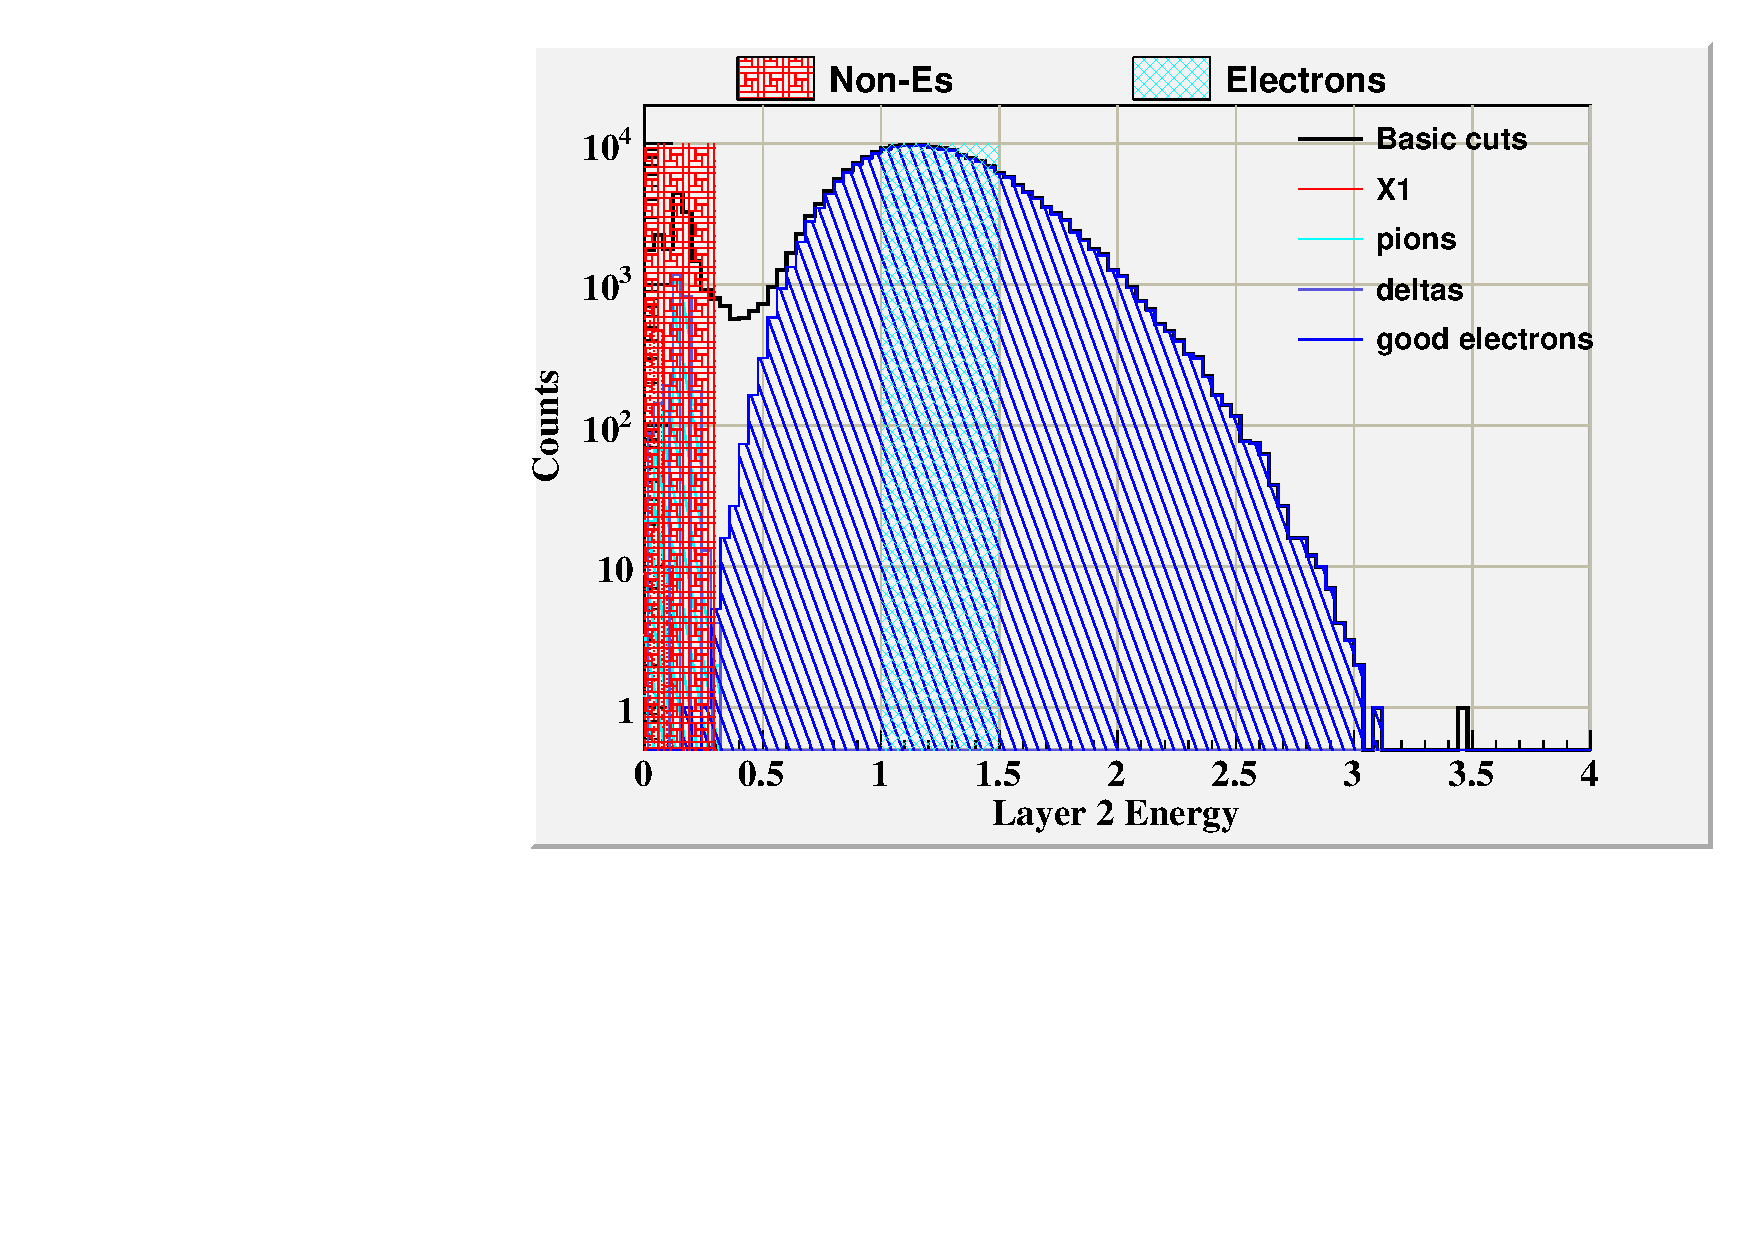
\includegraphics[width=4.50cm]{../images/Lprl2.pdf}
			\end{figure}
			\column{0.55\textwidth}
			Determine the Efficiency
			
			\begin{itemize}
				\item Electron sampling in two detectors
				\item Make threshold cut in the third
				\item Overall PID efficiency $> 98\% $
			\end{itemize}
			\vspace{-16pt}
			\begin{figure}
				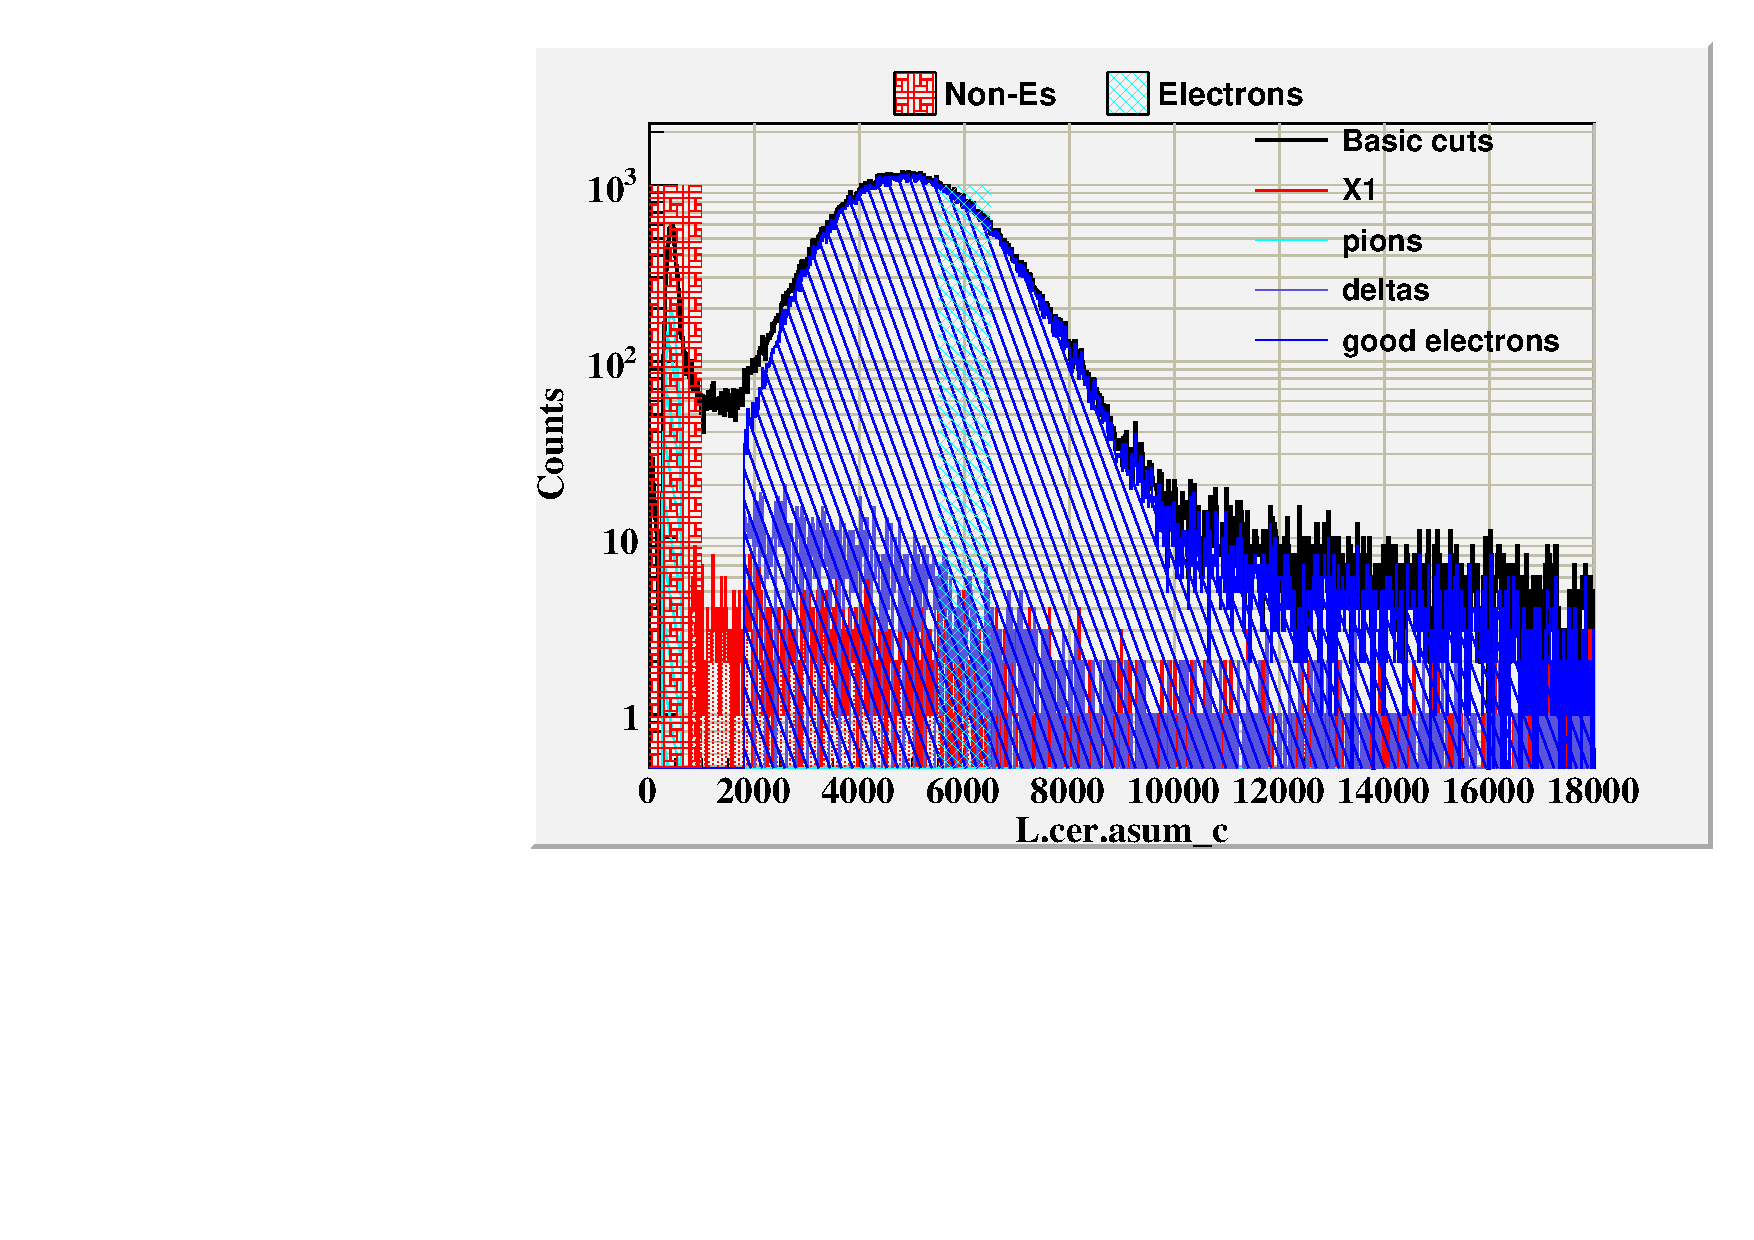
\includegraphics[width=5.50cm]{../images/Lcerasum.pdf}
			\end{figure}
			\vspace{-16pt}
			\textbf{Total cerenkov ADC signal with electron and non-electron sampling}
		\end{columns}
	\end{block}
\end{frame}
%------------------------------------------------------------------
\begin{frame}{Back Ground}
	\begin{block}{$\frac{Ne - \textbf{BG} }{Luminosity *  \epsilon}$}
		\begin{columns}
			\column{0.45\textwidth}
			\begin{itemize}
				\item Pion contamination
				\item Charge Symmetric background
			\end{itemize}
					\column{0.45\textwidth}
			\begin{itemize}
				\item End ap contamination
   				\item Beta decay of tritium
   			\end{itemize}
		\end{columns}	
		\begin{itemize}
			\item Pion contamination is corrected for via the PID efficiency  $ < 1\%$ 
			\item Beta Decay of Tritium to Helium was discussed by Tyler Kutz - Stony Brook University 
		\end{itemize}		
	\end{block}
\end{frame}
%------------------------------------------------------------------



\begin{frame}{End cap Contamination}
	\begin{block}{Contamination from Aluminum end caps}
		\begin{columns}
		\column{0.45\textwidth}
		\begin{itemize}
			\item Normalize end caps of Empty target to Gas filled target
			\item Normalized by measured thickness of end caps
			\item Scan Vertex Z location
			\item $3\%$ at low x$_{bj}$ for Helium-3 and Tritium
			\item Study by Tong Su and Tyler Hague
			\item images from Tong Su
		\end{itemize}
	
		\column{0.45\textwidth}
		\begin{figure}
			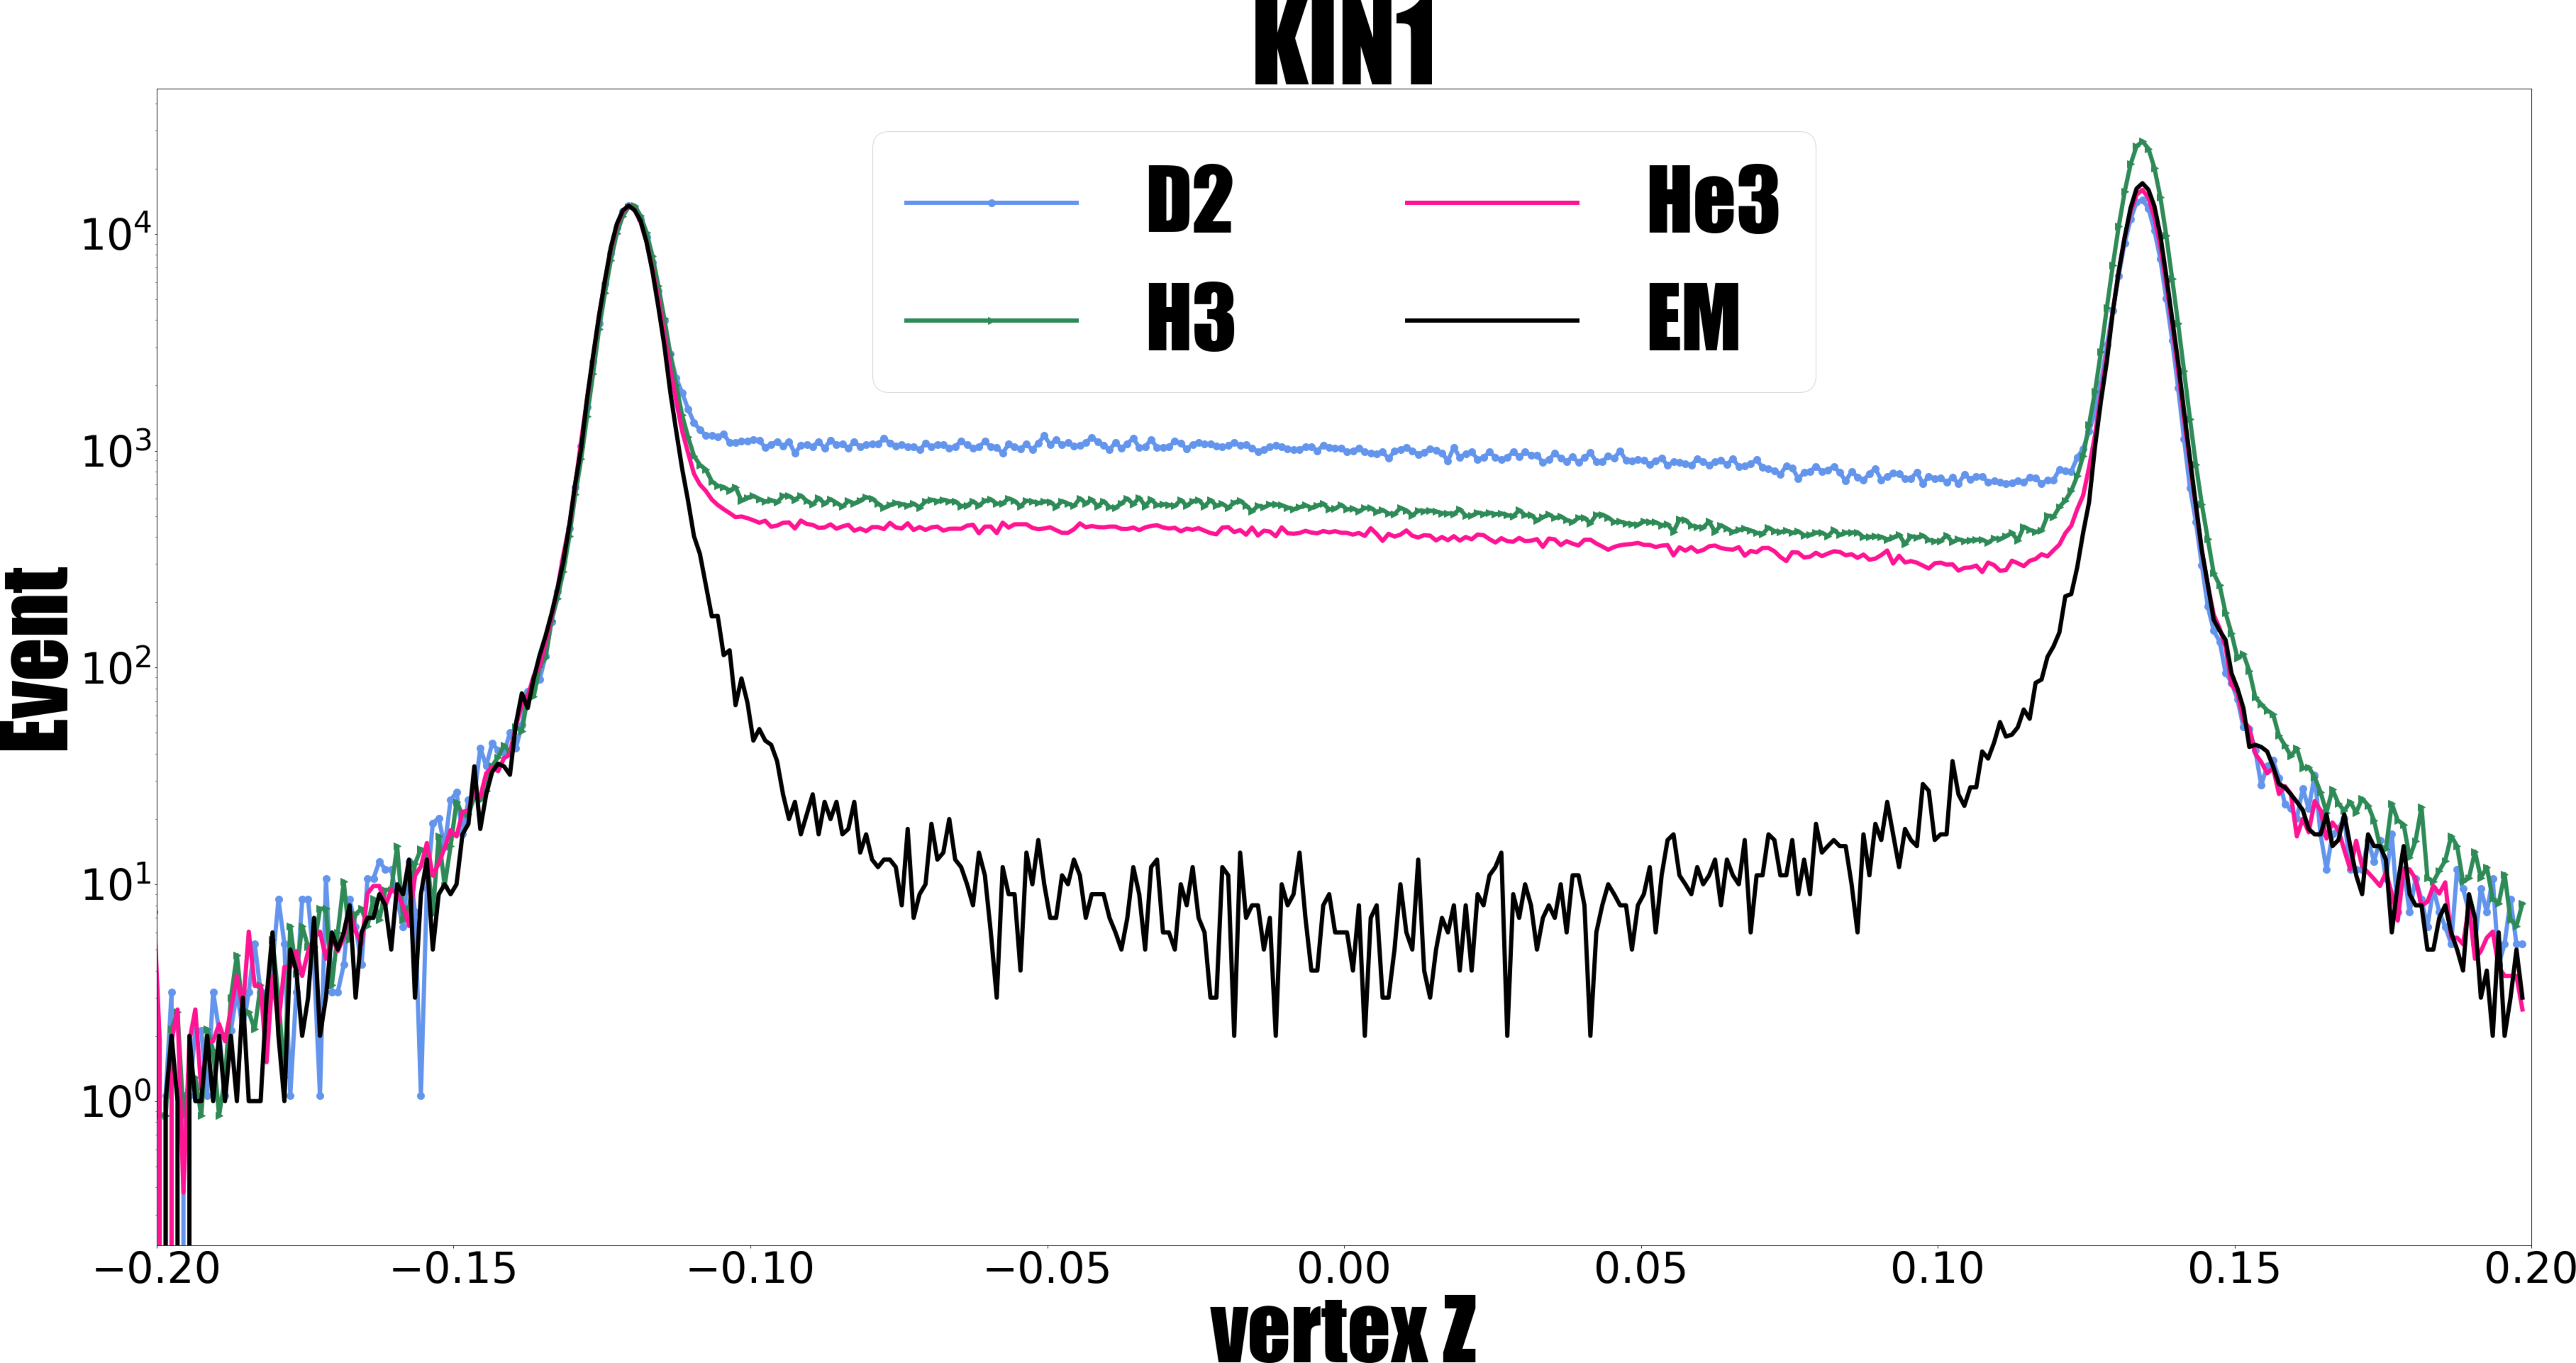
\includegraphics[width=5.0cm]{../images/ECC_kin1.pdf}
		\end{figure}
		\begin{figure}
			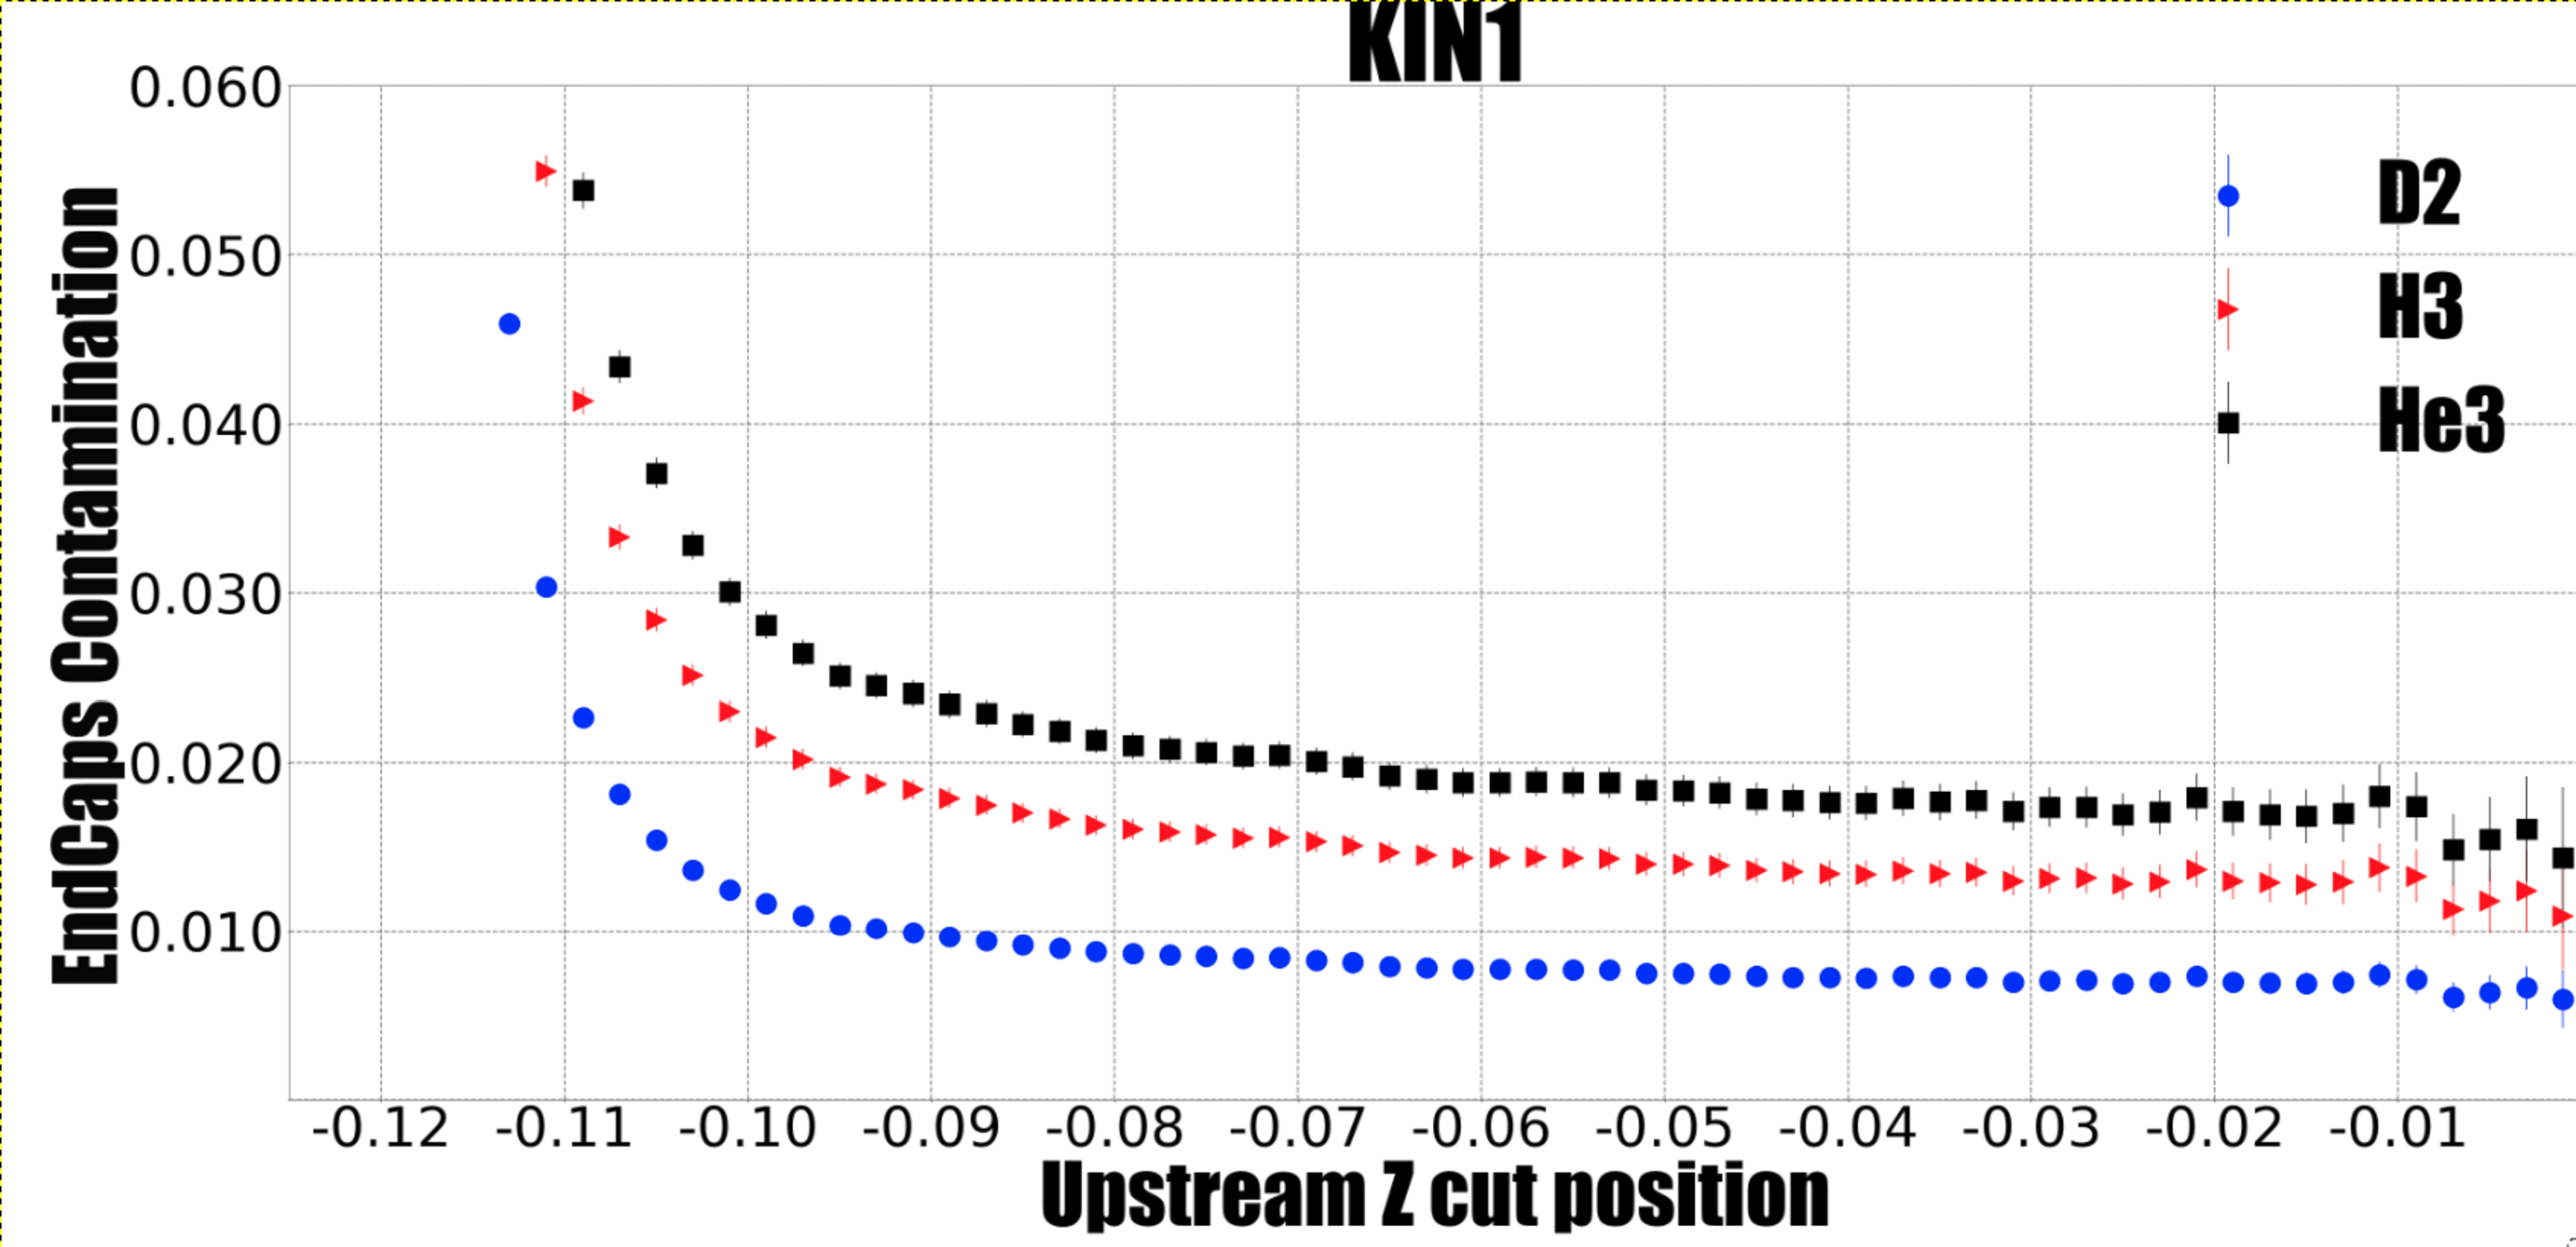
\includegraphics[width=5.0cm]{../images/ECC1_kin1.pdf}
		\end{figure}
	
		\end{columns}		
	\end{block}

\end{frame}

\begin{frame}{Charge Symmetric back ground}
\begin{block}{}
	\begin{columns}
		\column{0.45\textwidth}
		\begin{itemize}
			\item High energy photons decay into an e$^+$e$^-$ pairs
			\item Account for the pair produced e$^-$ by detecting the pair produced e$^+$
			\item Used HRS positive polarity settings at kinematics 1,2 and 3
			\item Fit results with an exponential function to determine the contamination factor at high $x_{Bj}$ kinematics.
			\item Images from Tong Su
		\end{itemize}
		\column{0.45\textwidth}
		\begin{figure}
			
		\end{figure}
		\vspace{-12pt}
		\begin{figure}
			\textbf{Tritium positron contamination}
			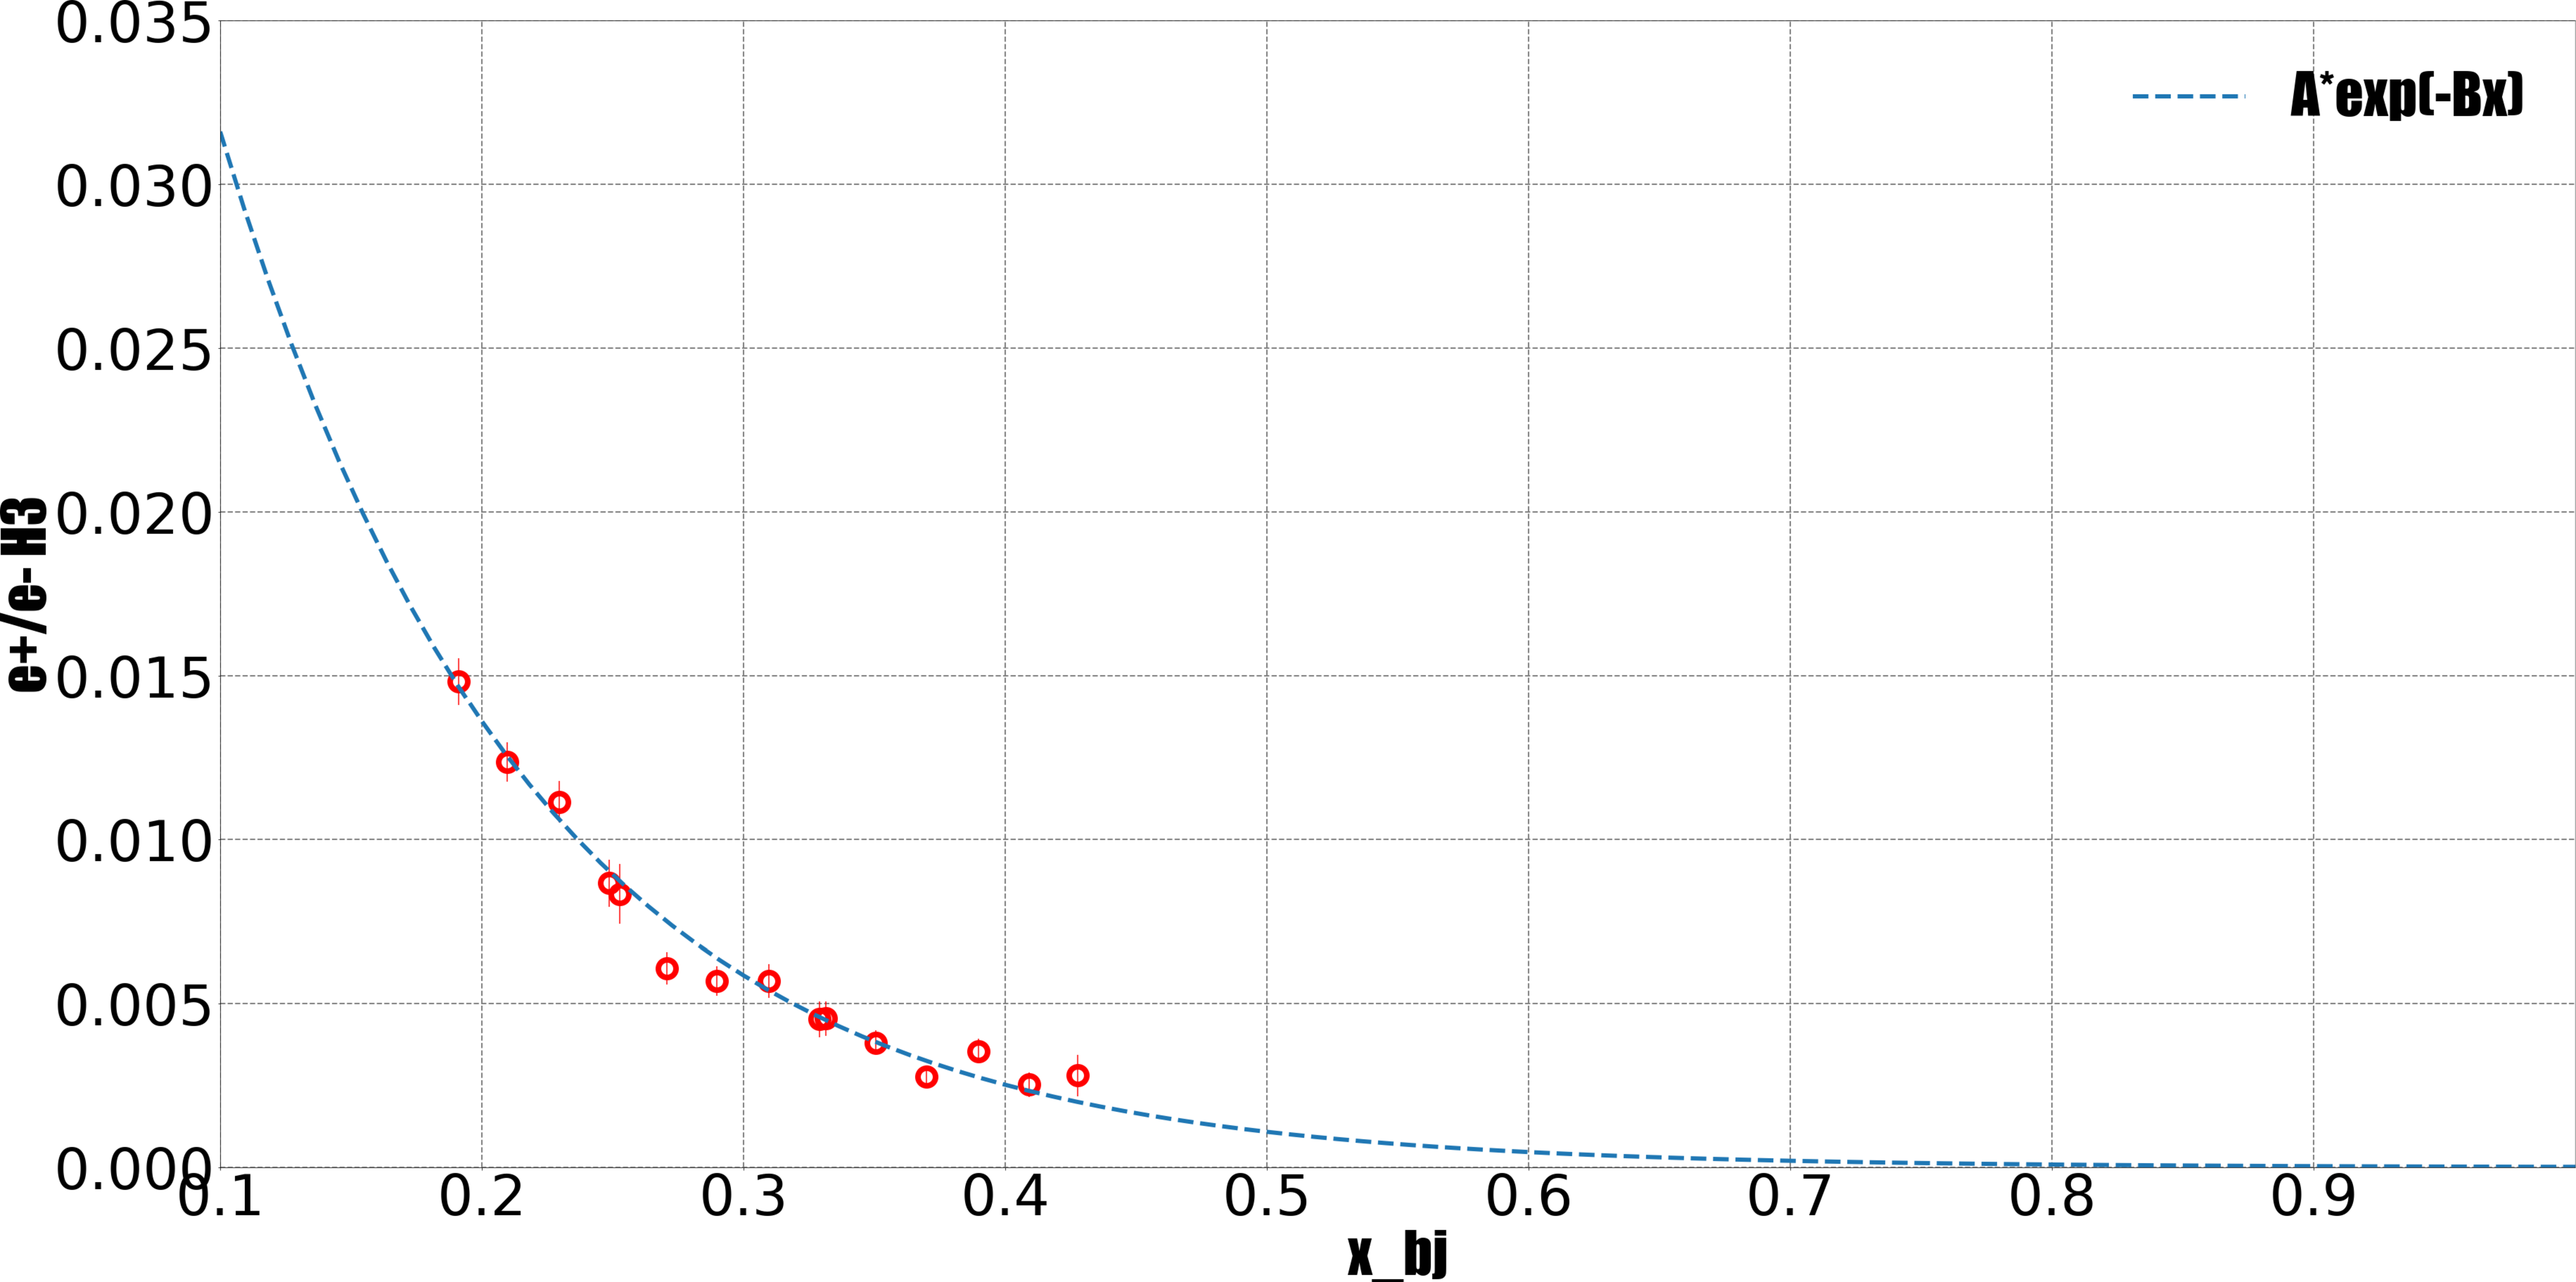
\includegraphics[width=5.0cm]{/home/jbane/images/positron_H3_bane.pdf}
		\end{figure}

	\end{columns}
	
\end{block}
\end{frame}

\begin{frame}{Monte Carlo Comparison}
		\vspace{-22pt}
	\begin{block}{Compare Monte Carlo to Data}
	 Spectrometer acceptance variables. 
		\vspace{-12pt}
		\begin{figure}[t]%
			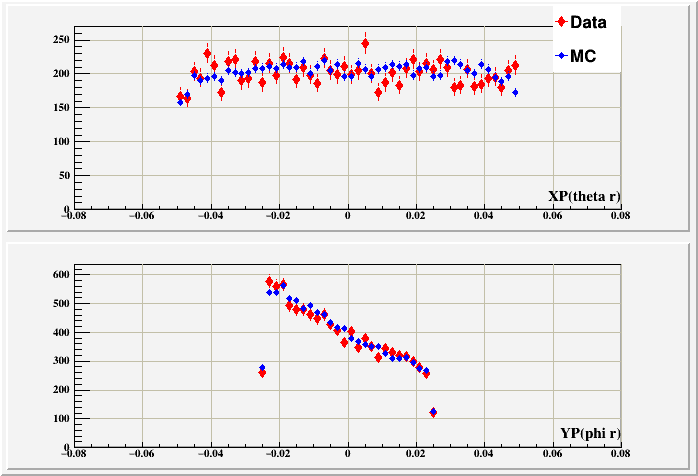
\includegraphics[width=5cm,height=5cm]{../images/xp_yp_tar_1207.png}
			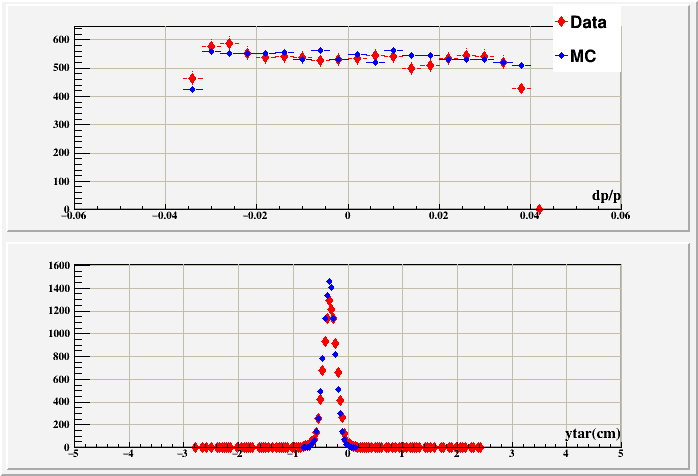
\includegraphics[width=5cm,height=5cm]{../images/dp_ytar_1207.png}
		\end{figure}
		\vspace{-12pt}	
		Top Left :theta(out of plane angle in rads from center)  Top Right: Dp/p(momentum from center).
		Bottom Left :phi(in plane angle in rads from center)  Top Right: Y target(vertex location in spectrometer coordinate frame).
	\end{block}	
\end{frame}

\begin{frame}{Cross section via monte carlo ratio}
\begin{block}{\textbf{Data to Monte Carlo ratio}}
	\begin{figure}
	\hspace*{-0.5cm}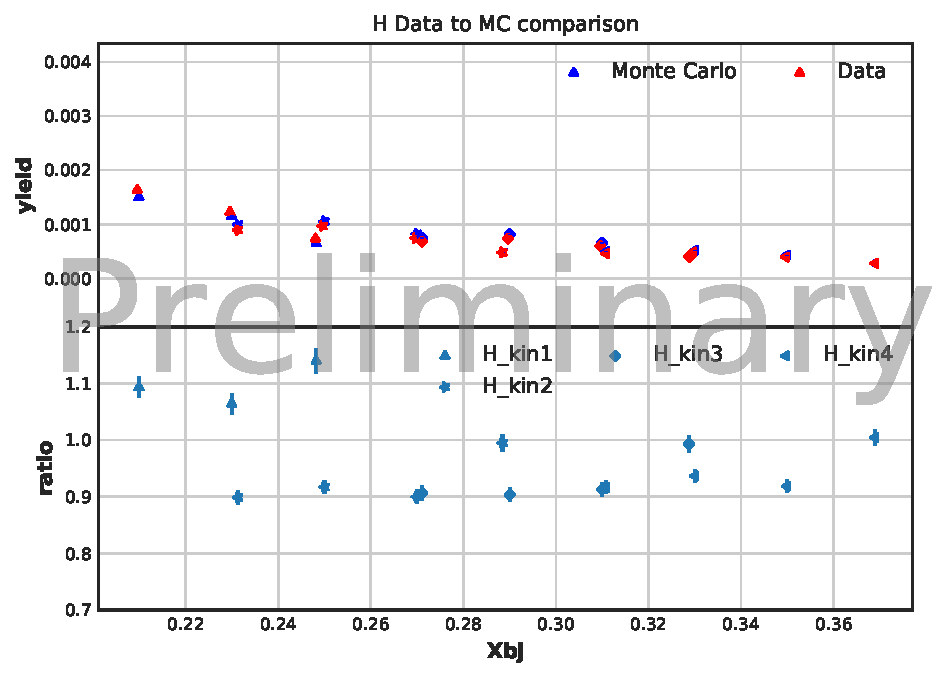
\includegraphics[height=5cm,width=5.50cm]{../images/H_all.pdf}			\hspace*{0.5cm}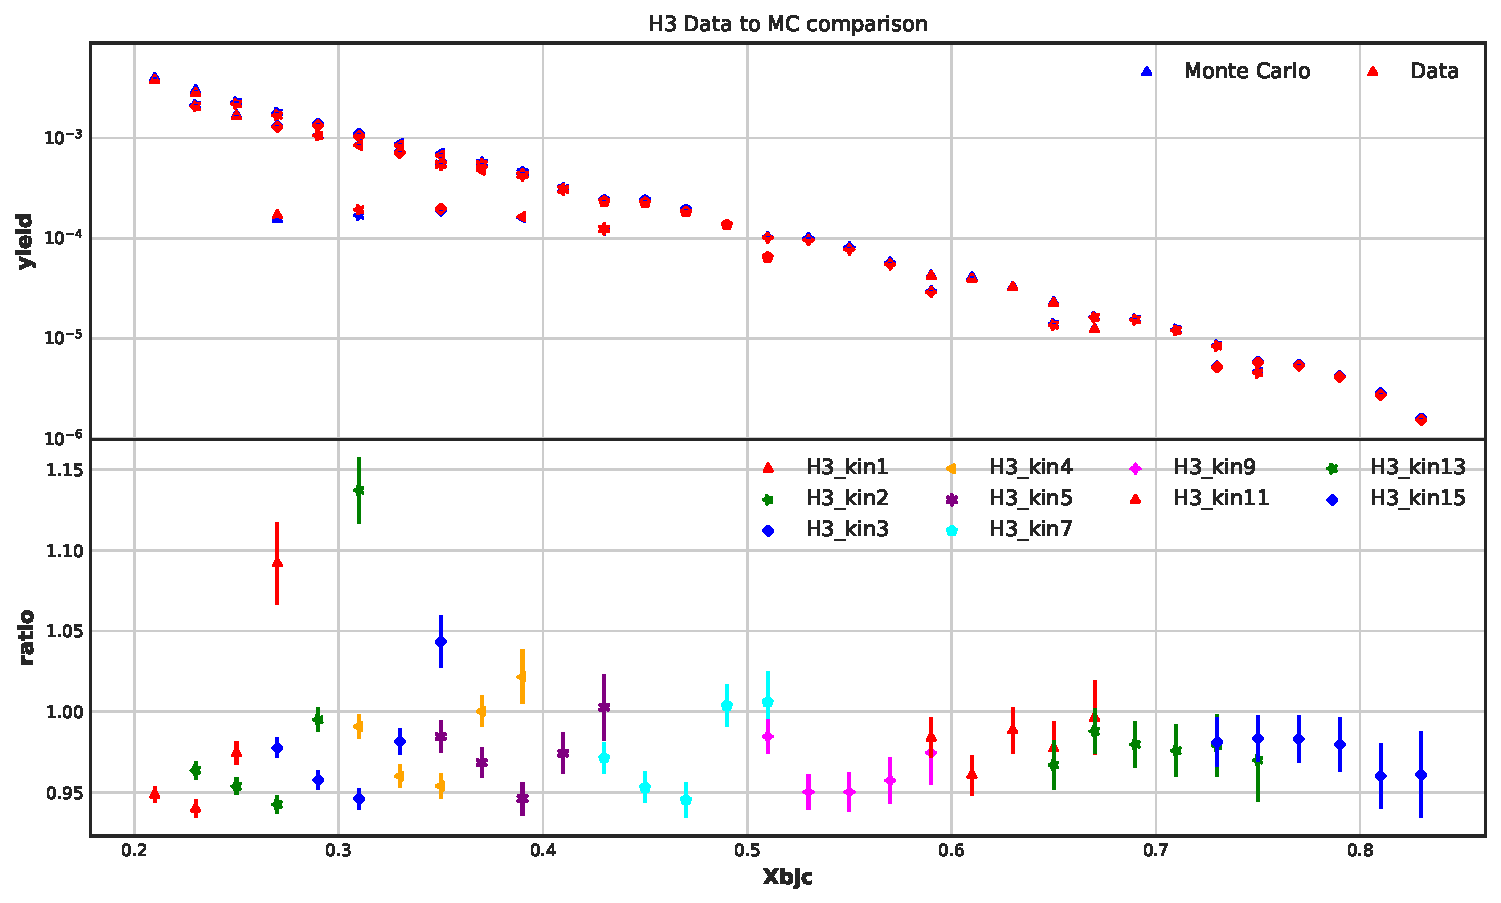
\includegraphics[height=5cm,width=5.50cm]{../images/H3_all.pdf}
	\end{figure}
\end{block}
\end{frame}

\begin{frame}{Cross section via monte carlo ratio}
\begin{block}{\textbf{Cross Section}}
	\begin{figure}
		\hspace*{-0.5cm}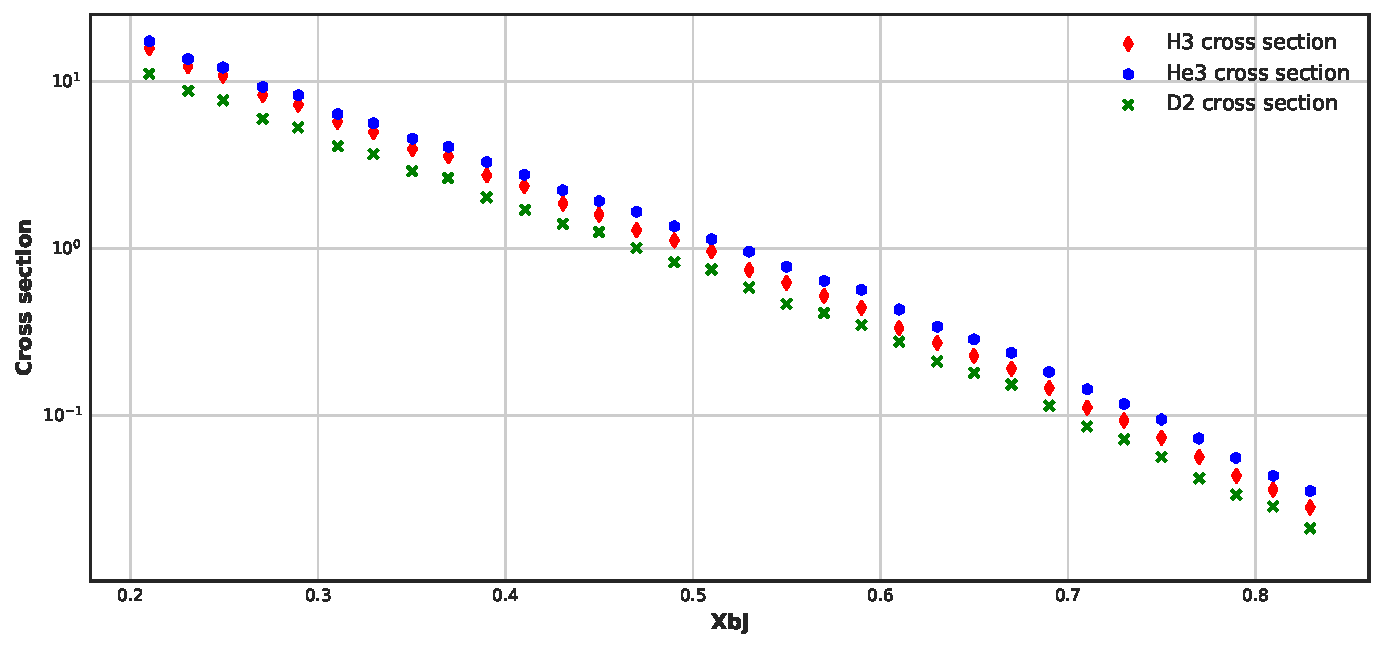
\includegraphics[height=5cm,width=10.50cm]{../images/multisigma.pdf}		
	\end{figure}
\end{block}
\end{frame}



\begin{frame}{Conclusion}
	\begin{block}{Task still in progress}
		\begin{itemize}
			\item Complete acceptance study and determine the systematics associated
			\item Study the systematic error from cross section model
			\item Finalize absolute cross section for helium-3, tritium, and deuterium 
			\item Study nuclear corrections and their systematics
			\item EMC effect for A=3 nuclei
		\end{itemize}
	\end{block}	
	\begin{block}{Special Thanks}
	\begin{itemize}
		\item JSA and University of Tennessee
		\item The MARATHON students
		\item The Tritium group 
		\item Hall A Collaboration
		\item Nadia Fomin and Doug Higinbotham
	\end{itemize}
\end{block}
\end{frame}
	
	


\end{document} 
